\documentclass[10pt]{beamer}
\usepackage[english]{babel}
\usepackage[utf8]{inputenc}
\usepackage[T1]{fontenc}
\usepackage{helvet}

%-------------------------------------------------------
% INFORMATION IN THE TITLE PAGE
%-------------------------------------------------------

\newcommand{\cstitle}{\textbf{Transformers meets neoantigen	detection: A systematics literature review}}
\subtitle[]{Jornadas de Investigación 2024}
\newcommand{\cscourseCode}{Matemáticas discretas II}
\newcommand{\csauthor}{Ph.D. Vicente Machaca Arceda}
\institute[UNSA]{Universidad de Ingeniería y Tecnología}
\newcommand{\csemail}{vmachaca@ulasalle.edu.pe}
\newcommand{\instituteabr}{ULASALLE}
\newcommand{\nameUp}{}
\date{2024}
\title[\cscourseCode]{\cstitle}
\author{\csauthor}
%%%%%%%%%%%%%%%%%

%-------------------------------------------------------
% CHOOSE THE THEME
%-------------------------------------------------------
\def\mycmd{0} % UNSA
\def\mycmd{1} % SALLE
\def\mycmd{2} % UTEC
\def\mycmd{3} % SALLE NEW
%-------------------------------------------------------


\if\mycmd0
\usepackage{csformat}
\newcommand{\chref}[3][blue]{\href{#2}{\color{#1}{#3}}}%

\fi

\if\mycmd1
\usetheme[]{Feather}
\newcommand{\chref}[2]{	\href{#1}{{\usebeamercolor[bg]{Feather}#2}} }
\fi

\if\mycmd2
\usetheme{UTEC2020}	
\newcommand{\chref}[3][blue]{\href{#2}{\color{#1}{#3}}}%
\fi

\if\mycmd3
\usetheme[]{SALLE}
\newcommand{\chref}[2]{	\href{#1}{{\usebeamercolor[bg]{Feather}#2}} }
\fi


\newcommand{\1}{
	\setbeamertemplate{background}{
		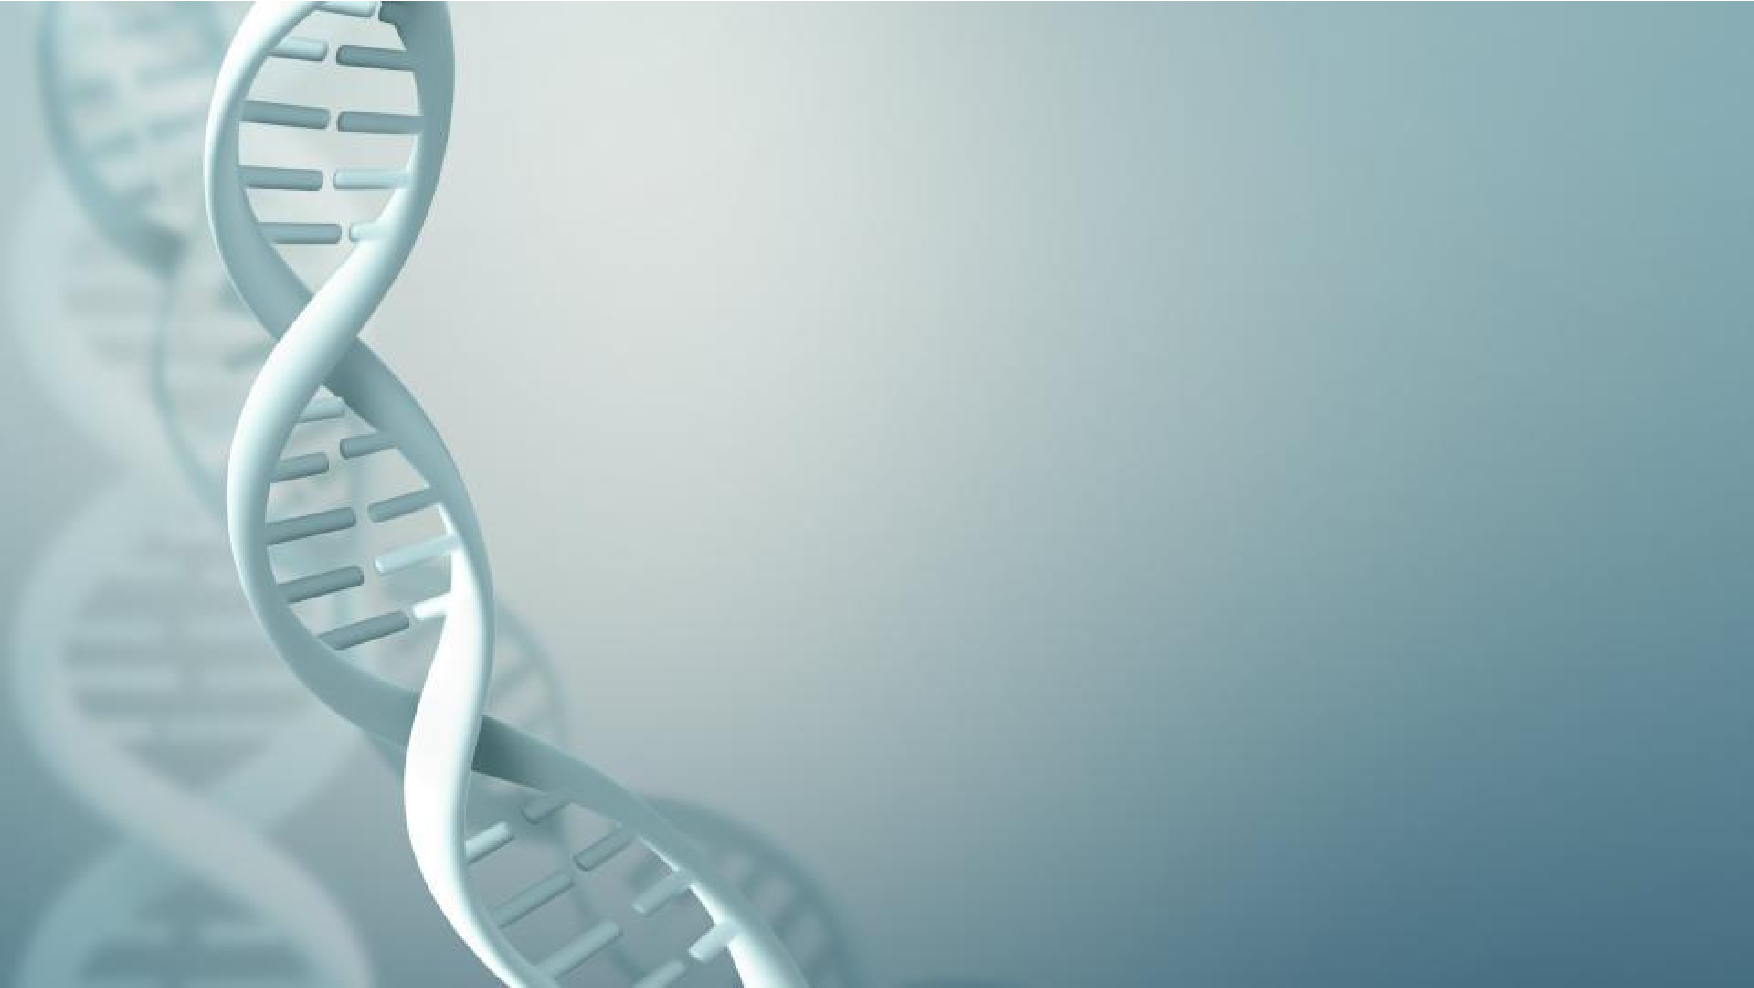
\includegraphics[width=\paperwidth,height=\paperheight]{../img/1}
		\tikz[overlay] \fill[fill opacity=0.75,fill=white] (0,0) rectangle (-\paperwidth,\paperheight);
	}
}



%-------------------------------------------------------
% THE BODY OF THE PRESENTATION
%-------------------------------------------------------

\begin{document}
	
	
	\AtBeginSubsection[]
	{
		\begin{frame}
			\frametitle{Content}
			\tableofcontents[currentsubsection]
		\end{frame}
	}
	
	
	%-------------------------------------------------------
	% THE TITLEPAGE
	%-------------------------------------------------------
	
	\if\mycmd0
	\maketitle
	\fi
	
	\if\mycmd1 % MY THEME
	\1{
		\begin{frame}[plain,noframenumbering] 
			\titlepage 
	\end{frame}}
	\fi
	
	\if\mycmd2
	\begin{frame}
		\titlepage
	\end{frame}
	\fi
	
	\if\mycmd3
	%\titlepage
	\begin{frame}[plain,noframenumbering] 
		\titlepage
	\end{frame}
	\fi
	%-------------------------------------------------------
	%-------------------------------------------------------

%-------------------------------------------------------
%-------------------------------------------------------
\begin{frame}{Contenido}
	\tableofcontents
\end{frame}
%-------------------------------------------------------
%-------------------------------------------------------


%%%%%%%%%%%%%%%%%%%%%%%%%%%%%%%%%%%%%%%%%%%%%%%%%%%%%%%%%%%%%%%%%%%%%%%%%%%%%%%%%%%%%%%%%%%%%%%%%%%%%%%%%%%%%%%%
%%%%%%%%%%%%%%%%%%%%%%%%%%%%%%%%%%%%%%%%%%%%%%%%%%%%%%%%%%%%%%%%%%%%%%%%%%%%%%%%%%%%%%%%%%%%%%%%%%%%%%%%%%%%%%%%
%%%%%%%%%%%%%%%%%%%%%%%%%%%%%%%%%%%%%%%%%%%%%%%%%%%%%%%%%%%%%%%%%%%%%%%%%%%%%%%%%%%%%%%%%%%%%%%%%%%%%%%%%%%%%%%%
\section{Marco teórico}
%%%%%%%%%%%%%%%%%%%%%%%%%%%%%%%%%%%%%%%%%%%%%%%%%%%%%%%%%%%%%%%%%%%%%%%%%%%%%%%%%%%%%%%%%%%%%%%%%%%%%%%%%%%%%%%%
%%%%%%%%%%%%%%%%%%%%%%%%%%%%%%%%%%%%%%%%%%%%%%%%%%%%%%%%%%%%%%%%%%%%%%%%%%%%%%%%%%%%%%%%%%%%%%%%%%%%%%%%%%%%%%%%
%%%%%%%%%%%%%%%%%%%%%%%%%%%%%%%%%%%%%%%%%%%%%%%%%%%%%%%%%%%%%%%%%%%%%%%%%%%%%%%%%%%%%%%%%%%%%%%%%%%%%%%%%%%%%%%%

%%%%%%%%%%%%%%%%%%%%%%%%%%%%%%%%%%%%%%%%%%%%%%%%%%%%%%%%%%%%%%%%%%%%%%%%%%%%%%%%%%%%%%%%%%%%%%%%%%%%%%%%%%%%%%%%
%%%%%%%%%%%%%%%%%%%%%%%%%%%%%%%%%%%%%%%%%%%%%%%%%%%%%%%%%%%%%%%%%%%%%%%%%%%%%%%%%%%%%%%%%%%%%%%%%%%%%%%%%%%%%%%%
%%%%%%%%%%%%%%%%%%%%%%%%%%%%%%%%%%%%%%%%%%%%%%%%%%%%%%%%%%%%%%%%%%%%%%%%%%%%%%%%%%%%%%%%%%%%%%%%%%%%%%%%%%%%%%%%
\subsection{Bioinformática y DNA}
%%%%%%%%%%%%%%%%%%%%%%%%%%%%%%%%%%%%%%%%%%%%%%%%%%%%%%%%%%%%%%%%%%%%%%%%%%%%%%%%%%%%%%%%%%%%%%%%%%%%%%%%%%%%%%%%
%%%%%%%%%%%%%%%%%%%%%%%%%%%%%%%%%%%%%%%%%%%%%%%%%%%%%%%%%%%%%%%%%%%%%%%%%%%%%%%%%%%%%%%%%%%%%%%%%%%%%%%%%%%%%%%%
%%%%%%%%%%%%%%%%%%%%%%%%%%%%%%%%%%%%%%%%%%%%%%%%%%%%%%%%%%%%%%%%%%%%%%%%%%%%%%%%%%%%%%%%%%%%%%%%%%%%%%%%%%%%%%%%

%-------------------------------------------------------
%-------------------------------------------------------
\begin{frame}{Bioinformática}{}		
	\begin{figure}
		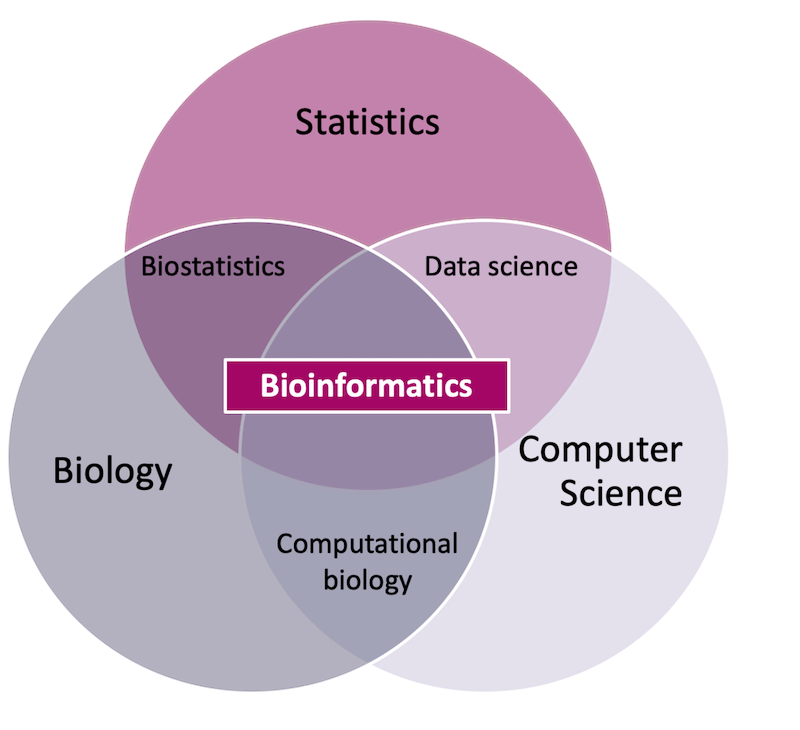
\includegraphics[width=0.7\textwidth]{../img/neoantigen/bioinformatics2}
		
	\end{figure}		
\end{frame}
%-------------------------------------------------------
%-------------------------------------------------------

%-------------------------------------------------------
%-------------------------------------------------------
\begin{frame}{DNA}{Localización}
	\begin{figure}[]
		\centering
		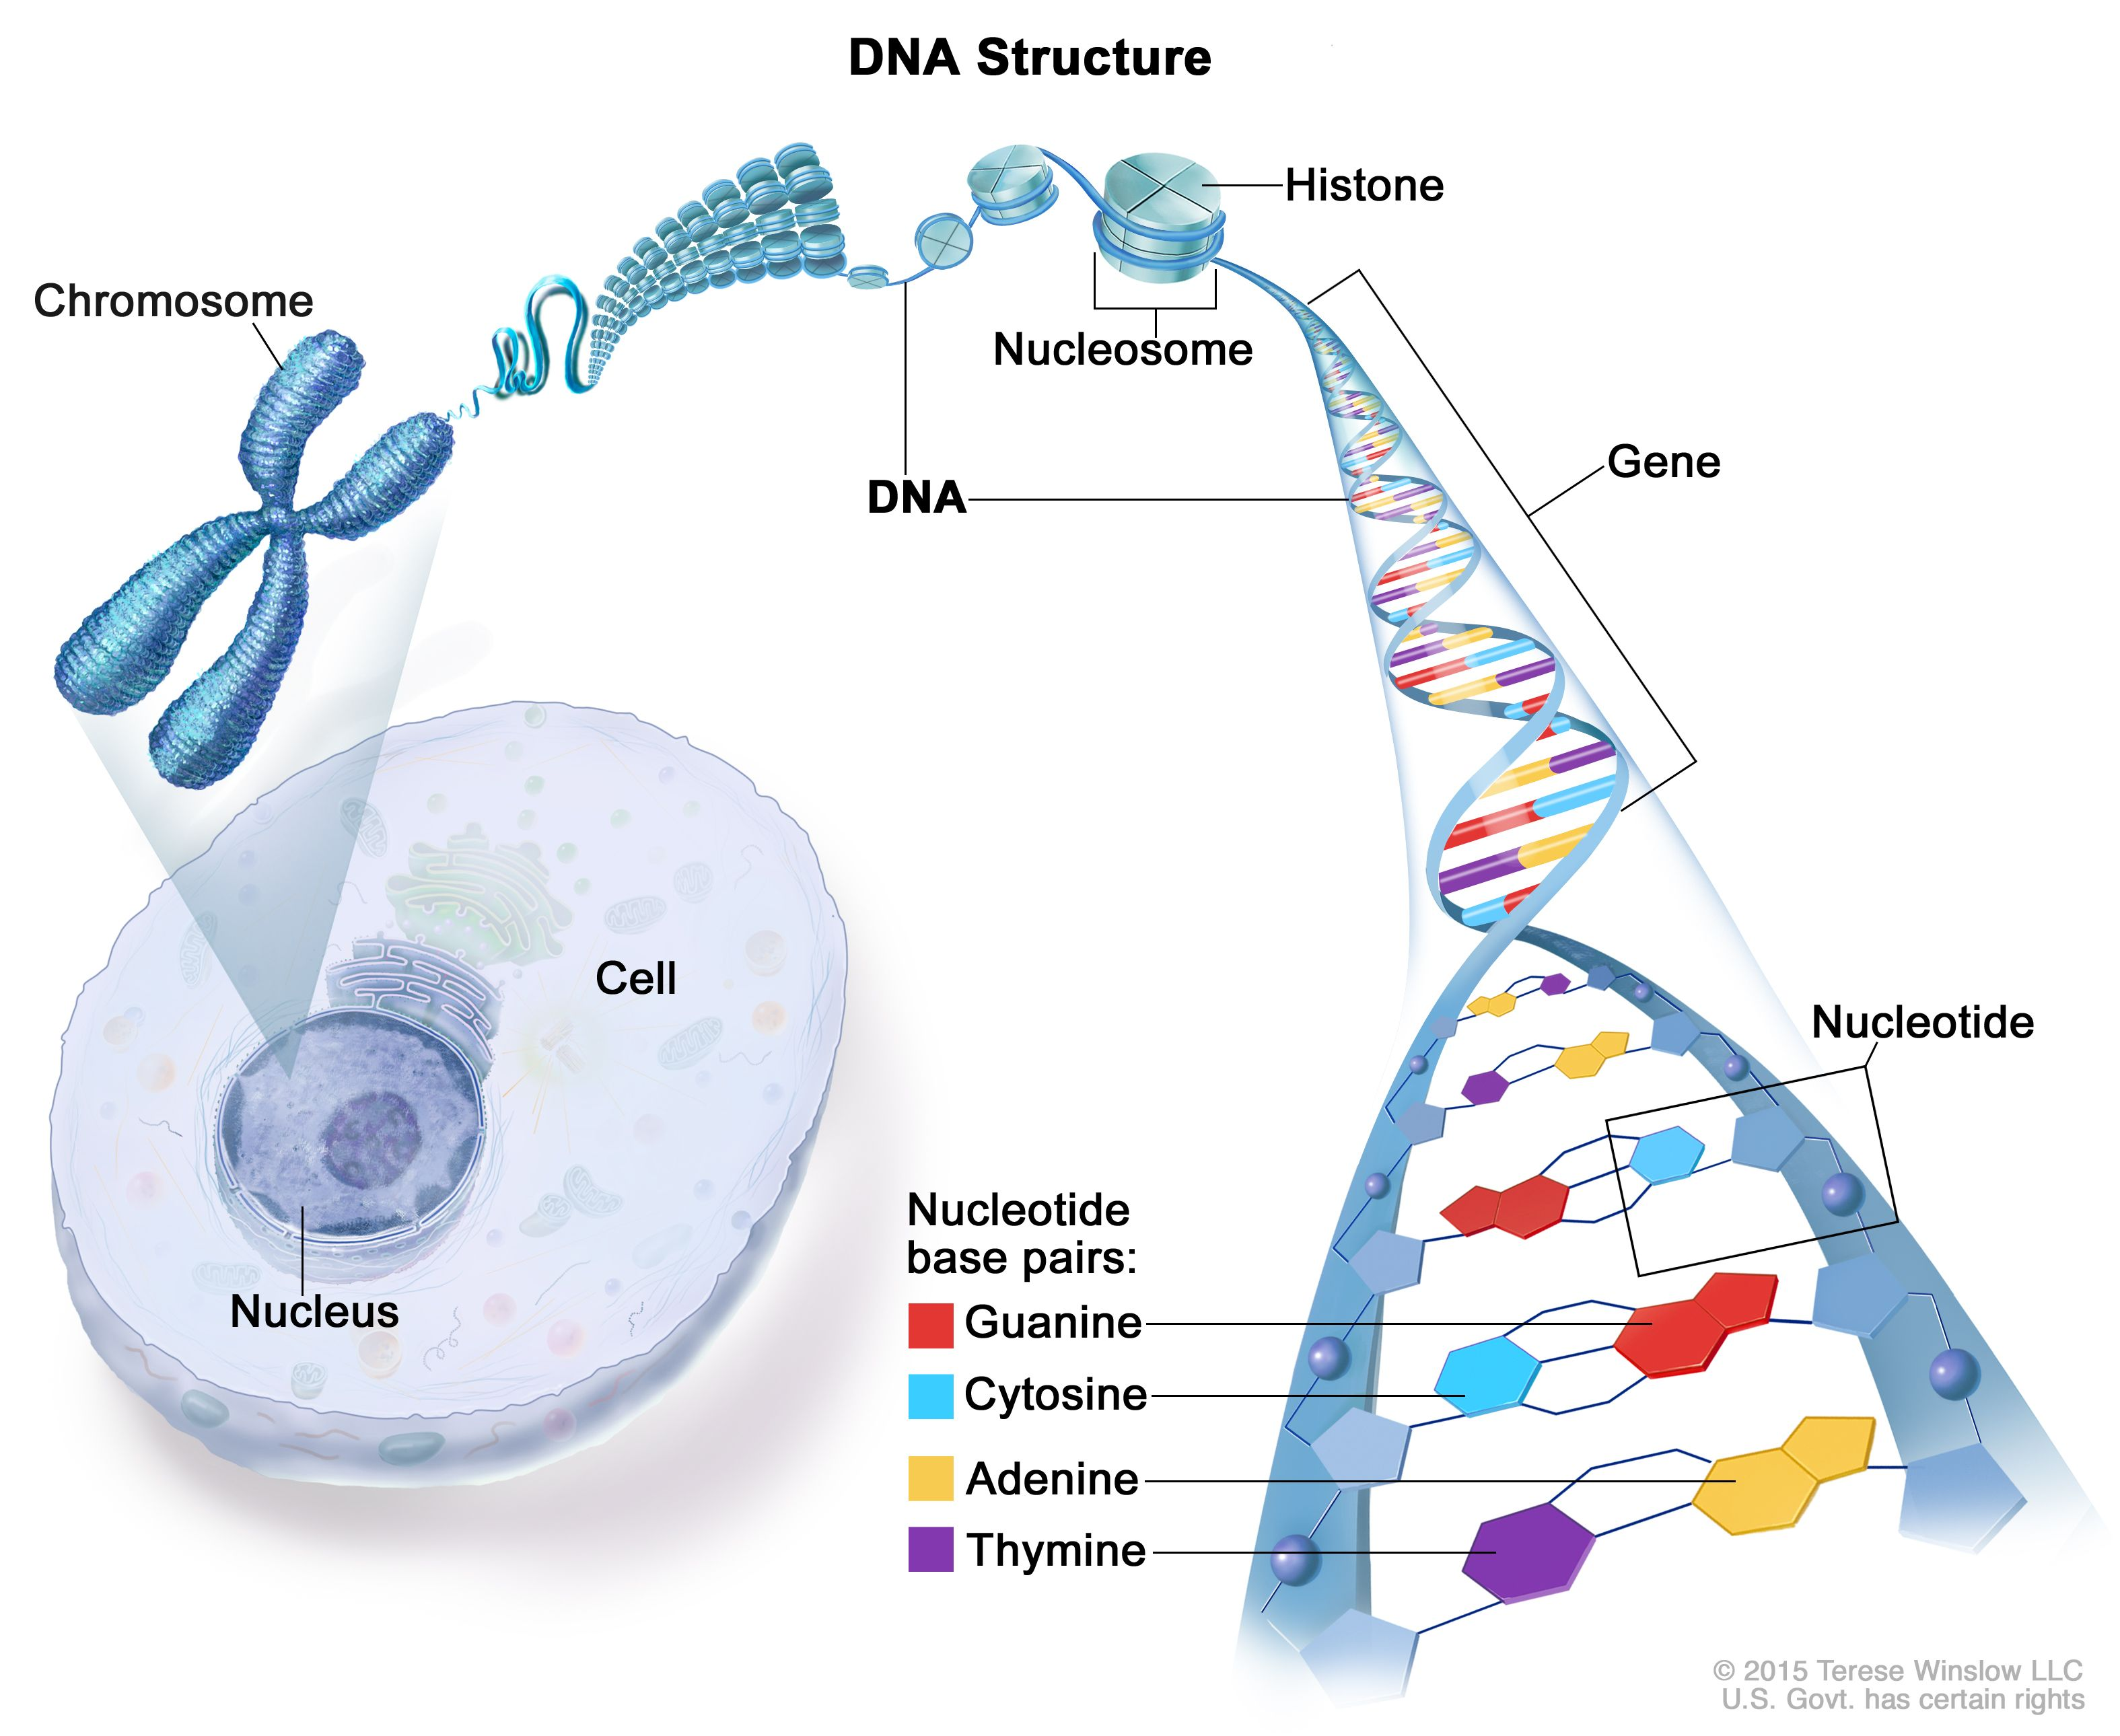
\includegraphics[width=\textwidth,height=0.65\textheight,keepaspectratio]{../img/neoantigen/dna}
		\label{img:mot2}
		\caption{Where DNA is located \cite{NCIdictionary2022}.}
	\end{figure}
\end{frame}
%-------------------------------------------------------
%-------------------------------------------------------

%-------------------------------------------------------
%-------------------------------------------------------
\begin{frame}{DNA}{Ejemplo}
	\begin{figure}[]
		\centering
		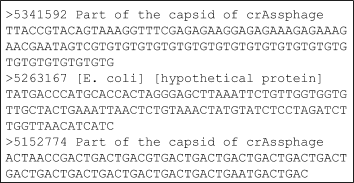
\includegraphics[width=\textwidth,height=0.65\textheight,keepaspectratio]{../img/neoantigen/DNA_sample}		
	\end{figure}
\end{frame}
%-------------------------------------------------------
%-------------------------------------------------------



%-------------------------------------------------------
%-------------------------------------------------------
\begin{frame}{DNA}{De DNA a proteínas}
	\begin{figure}[]
		\centering
		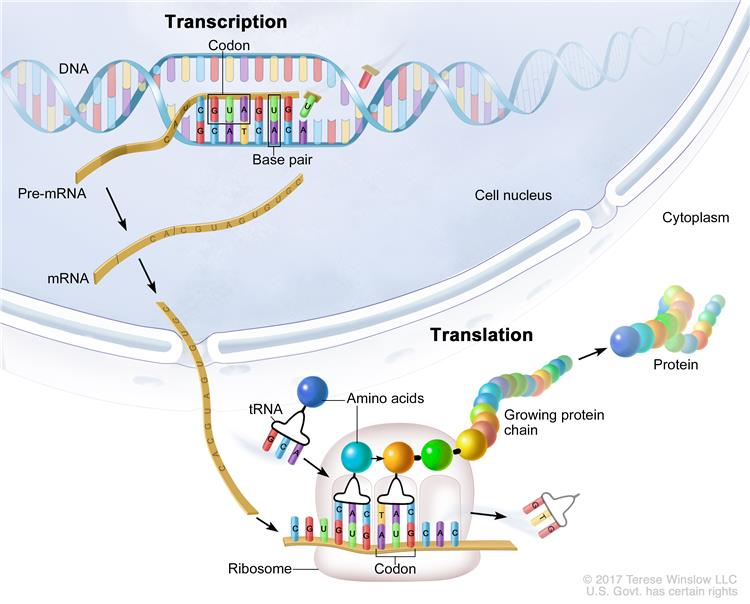
\includegraphics[width=0.7\textwidth]{../img/neoantigen/trans.jpg}
		\caption{Transcription and translation \cite{nci2020}.}
	\end{figure}
\end{frame}
%-------------------------------------------------------
%-------------------------------------------------------

%%%%%%%%%%%%%%%%%%%%%%%%%%%%%%%%%%%%%%%%%%%%%%%%%%%%%%%%%%%%%%%%%%%%%%%%%%%%%%%%%%%%%%%%%%%%%%%%%%%%%%%%%%%%%%%%
%%%%%%%%%%%%%%%%%%%%%%%%%%%%%%%%%%%%%%%%%%%%%%%%%%%%%%%%%%%%%%%%%%%%%%%%%%%%%%%%%%%%%%%%%%%%%%%%%%%%%%%%%%%%%%%%
%%%%%%%%%%%%%%%%%%%%%%%%%%%%%%%%%%%%%%%%%%%%%%%%%%%%%%%%%%%%%%%%%%%%%%%%%%%%%%%%%%%%%%%%%%%%%%%%%%%%%%%%%%%%%%%%
\subsection{Mutaciones}
%%%%%%%%%%%%%%%%%%%%%%%%%%%%%%%%%%%%%%%%%%%%%%%%%%%%%%%%%%%%%%%%%%%%%%%%%%%%%%%%%%%%%%%%%%%%%%%%%%%%%%%%%%%%%%%%
%%%%%%%%%%%%%%%%%%%%%%%%%%%%%%%%%%%%%%%%%%%%%%%%%%%%%%%%%%%%%%%%%%%%%%%%%%%%%%%%%%%%%%%%%%%%%%%%%%%%%%%%%%%%%%%%
%%%%%%%%%%%%%%%%%%%%%%%%%%%%%%%%%%%%%%%%%%%%%%%%%%%%%%%%%%%%%%%%%%%%%%%%%%%%%%%%%%%%%%%%%%%%%%%%%%%%%%%%%%%%%%%%

%-------------------------------------------------------
%-------------------------------------------------------
\begin{frame}{Variantes y Mutaciones}{Tipos}
	\begin{block}{}
		\begin{itemize}
			\item \textbf{\textit{Single-Nucleotide Variant} (SNV)}, cambios a menos de 10 bases.
			\item \textbf{\textit{Structural Variation} (SV)}, cambios a mas de 10 bases, incluso pueden llegar a aumentar la cantidad de cromosomas.
		\end{itemize}	
	\end{block}
\end{frame}
%-------------------------------------------------------
%-------------------------------------------------------

%-------------------------------------------------------
%-------------------------------------------------------
\begin{frame}{Variantes y Mutaciones}{Ejemplo}
	\begin{figure}[]
		\centering
		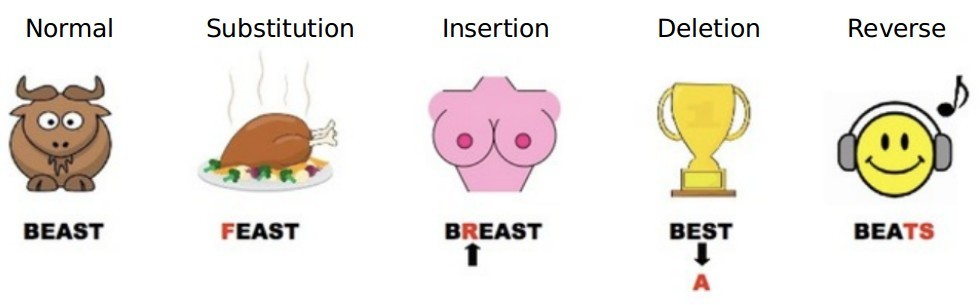
\includegraphics[width=\textwidth,height=0.7\textheight,keepaspectratio]{../img/neoantigen/point_mutations_med.jpg}
		\label{img:alig}
		\caption{Overview of the Different Types of Point Mutations.}
	\end{figure}
\end{frame}
%-------------------------------------------------------
%-------------------------------------------------------

%-------------------------------------------------------
%-------------------------------------------------------
\begin{frame}{Variantes y Mutaciones}{}
	\begin{figure}[h]
		\centering
		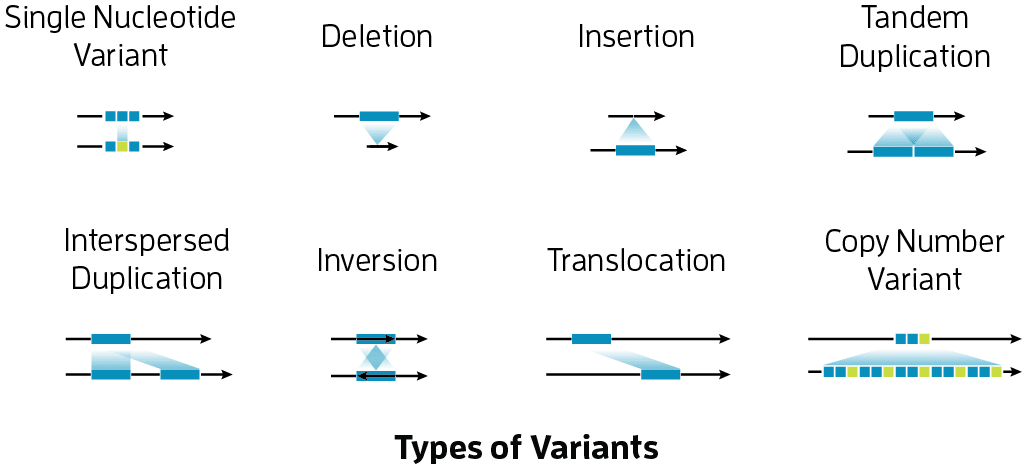
\includegraphics[width=\textwidth]{../img/neoantigen/variants}
		\caption{Example of structural variants. Source: \cite{sv_pacbio_2021}}
		\label{fig:variants}
	\end{figure}	
\end{frame}
%-------------------------------------------------------
%-------------------------------------------------------


%-------------------------------------------------------
%-------------------------------------------------------
\begin{frame}{Variaciones a nivel de cromosomas}{}
	\begin{figure}
		\centering
		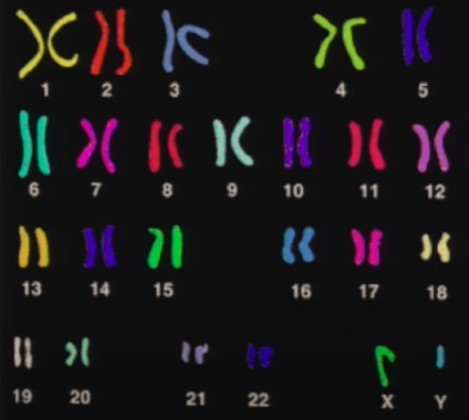
\includegraphics[width=0.6\textwidth]{../img/neoantigen/chrom}
		\caption{Los 46 cromosomas presentes en una célula.}
	\end{figure}		
\end{frame}
%-------------------------------------------------------
%-------------------------------------------------------

%-------------------------------------------------------
%-------------------------------------------------------
\begin{frame}{Variaciones a nivel de cromosomas}{}
	\begin{figure}
		\centering
		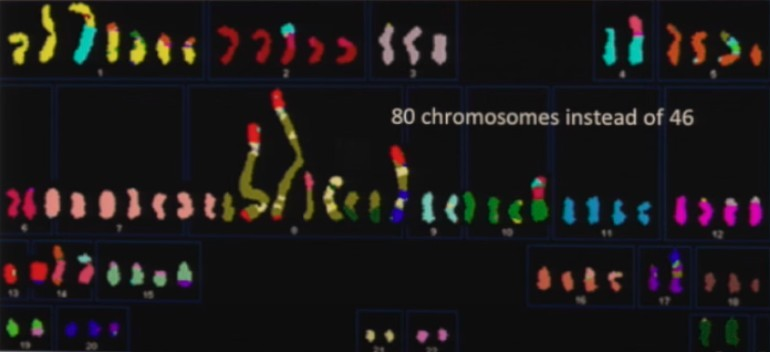
\includegraphics[width=\textwidth]{../img/neoantigen/chrom3}
		\caption{Cromosomas de una mujer con Cáncer de mama (1971).}
	\end{figure}		
\end{frame}
%-------------------------------------------------------
%-------------------------------------------------------

%%%%%%%%%%%%%%%%%%%%%%%%%%%%%%%%%%%%%%%%%%%%%%%%%%%%%%%%%%%%%%%%%%%%%%%%%%%%%%%%%%%%%%%%%%%%%%%%%%%%%%%%%%%%%%%%
%%%%%%%%%%%%%%%%%%%%%%%%%%%%%%%%%%%%%%%%%%%%%%%%%%%%%%%%%%%%%%%%%%%%%%%%%%%%%%%%%%%%%%%%%%%%%%%%%%%%%%%%%%%%%%%%
%%%%%%%%%%%%%%%%%%%%%%%%%%%%%%%%%%%%%%%%%%%%%%%%%%%%%%%%%%%%%%%%%%%%%%%%%%%%%%%%%%%%%%%%%%%%%%%%%%%%%%%%%%%%%%%%
\subsection{Neo antígenos}
%%%%%%%%%%%%%%%%%%%%%%%%%%%%%%%%%%%%%%%%%%%%%%%%%%%%%%%%%%%%%%%%%%%%%%%%%%%%%%%%%%%%%%%%%%%%%%%%%%%%%%%%%%%%%%%%
%%%%%%%%%%%%%%%%%%%%%%%%%%%%%%%%%%%%%%%%%%%%%%%%%%%%%%%%%%%%%%%%%%%%%%%%%%%%%%%%%%%%%%%%%%%%%%%%%%%%%%%%%%%%%%%%
%%%%%%%%%%%%%%%%%%%%%%%%%%%%%%%%%%%%%%%%%%%%%%%%%%%%%%%%%%%%%%%%%%%%%%%%%%%%%%%%%%%%%%%%%%%%%%%%%%%%%%%%%%%%%%%%

%-------------------------------------------------------
%-------------------------------------------------------
\begin{frame}{Inmunoterapia del Cáncer}{}		
	Es un tipo de tratamiento contra el Cáncer que estimula las defensas naturales del cuerpo para combatir el Cáncer \cite{inmunoterapy2022}.
		
	\begin{figure}
		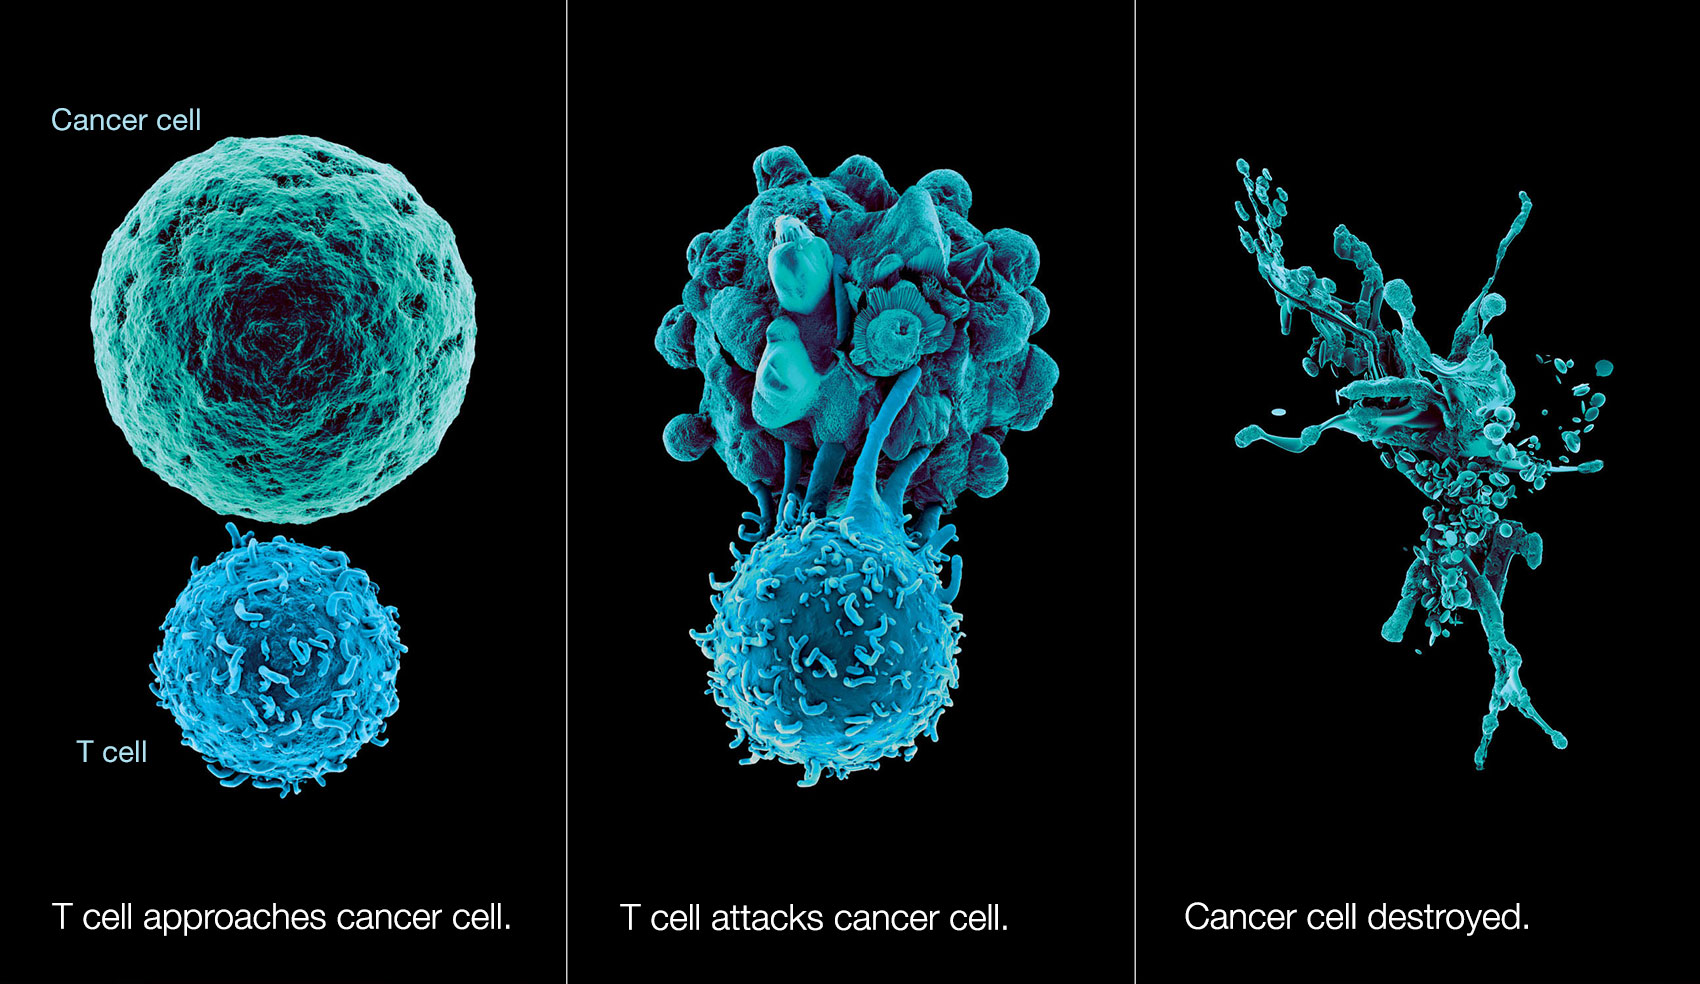
\includegraphics[width=0.85\textwidth]{../img/neoantigen/tcell}
		\caption{Ejemplo de como una célula T destruye células del cancer \cite{nortshore2022}.}
	\end{figure}		
\end{frame}
%-------------------------------------------------------
%-------------------------------------------------------

%-------------------------------------------------------
%-------------------------------------------------------
\begin{frame}{Inmunoterapia del Cáncer}{Neo antígenos}		
	\begin{block}{}
		Es una \textbf{proteína} que se forma en las células de Cáncer cuando ocurre mutaciones en el DNA, cumplen un rol importante al \textbf{estimular una respuesta inmune} \cite{NCIdictionary2022, borden2022cancer}.
	\end{block} 
	\begin{block}{}
		En la actualidad hay varios métodos para detectar a predecir neo antígenos, pero \textbf{solo una pequeña cantidad de ellos} logran estimular al sistema inmune \cite{chen2021challenges, hao2021improvement}.
	\end{block}
\end{frame}
%-------------------------------------------------------
%-------------------------------------------------------

%-------------------------------------------------------
%-------------------------------------------------------
\begin{frame}{Inmunoterapia del Cáncer}{Generación de vacunas}	
	\begin{figure}
		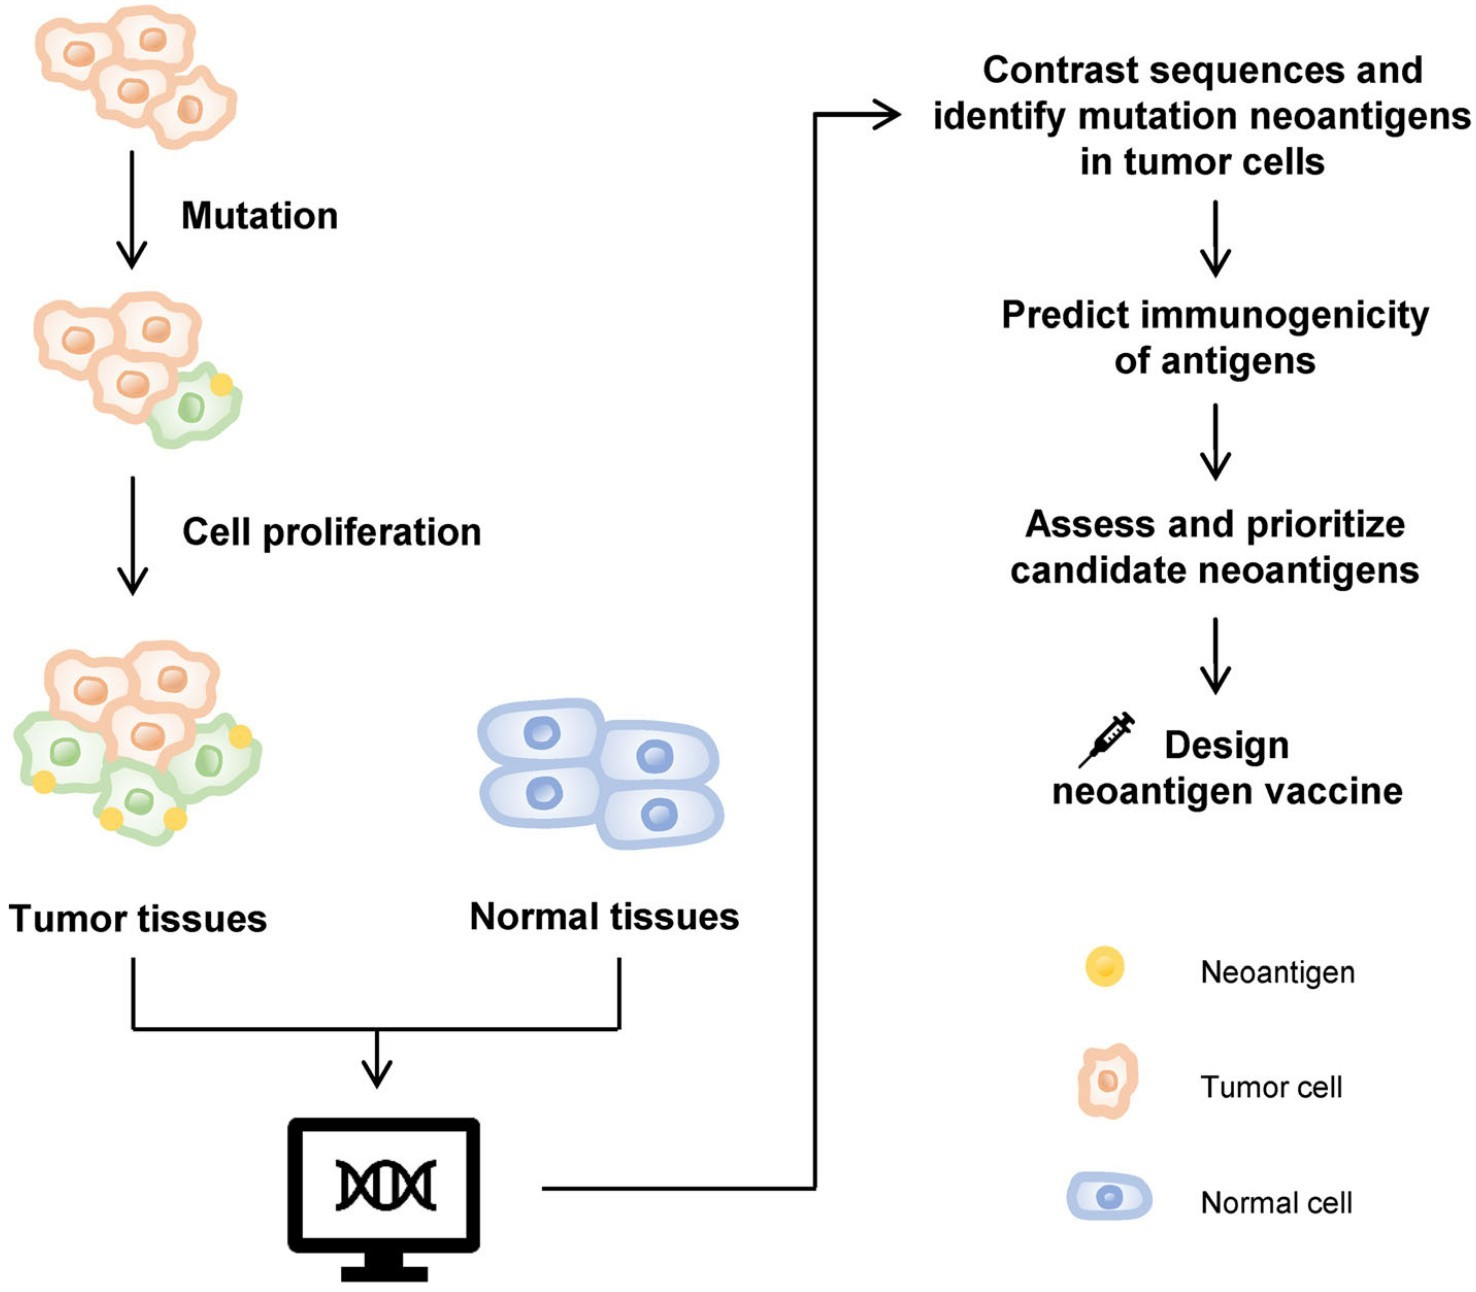
\includegraphics[width=0.6\textwidth]{../img/neoantigen/process}
		\caption{Proceso para la generación de vacunas personalizadas \cite{peng2019neoantigen}.}
	\end{figure}		
\end{frame}
%-------------------------------------------------------
%-------------------------------------------------------



%%%%%%%%%%%%%%%%%%%%%%%%%%%%%%%%%%%%%%%%%%%%%%%%%%%%%%%%%%%%%%%%%%%%%%%%%%%%%%%%%%%%%%%%%%%%%%%%%%%%%%%%%%%%%%%%
%%%%%%%%%%%%%%%%%%%%%%%%%%%%%%%%%%%%%%%%%%%%%%%%%%%%%%%%%%%%%%%%%%%%%%%%%%%%%%%%%%%%%%%%%%%%%%%%%%%%%%%%%%%%%%%%
%%%%%%%%%%%%%%%%%%%%%%%%%%%%%%%%%%%%%%%%%%%%%%%%%%%%%%%%%%%%%%%%%%%%%%%%%%%%%%%%%%%%%%%%%%%%%%%%%%%%%%%%%%%%%%%%
\subsection{Transformers}
%%%%%%%%%%%%%%%%%%%%%%%%%%%%%%%%%%%%%%%%%%%%%%%%%%%%%%%%%%%%%%%%%%%%%%%%%%%%%%%%%%%%%%%%%%%%%%%%%%%%%%%%%%%%%%%%
%%%%%%%%%%%%%%%%%%%%%%%%%%%%%%%%%%%%%%%%%%%%%%%%%%%%%%%%%%%%%%%%%%%%%%%%%%%%%%%%%%%%%%%%%%%%%%%%%%%%%%%%%%%%%%%%
%%%%%%%%%%%%%%%%%%%%%%%%%%%%%%%%%%%%%%%%%%%%%%%%%%%%%%%%%%%%%%%%%%%%%%%%%%%%%%%%%%%%%%%%%%%%%%%%%%%%%%%%%%%%%%%%


%-------------------------------------------------------
%-------------------------------------------------------
\begin{frame}{Transformers}{}	
	\begin{figure}
		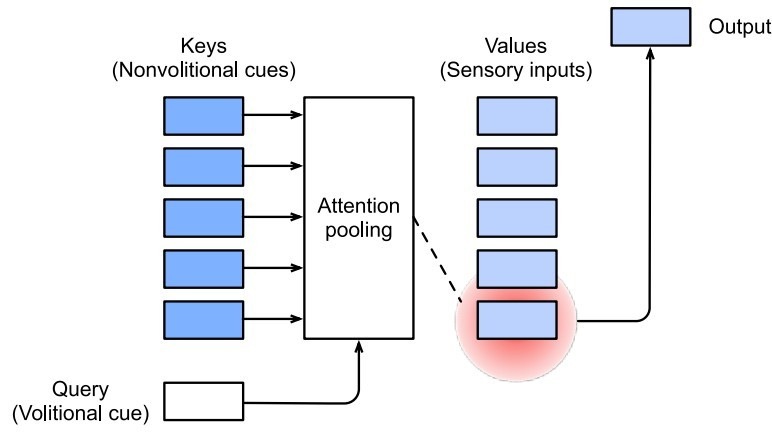
\includegraphics[width=0.9\textwidth]{../img/neoantigen/transformer}
	\end{figure}		
\end{frame}
%-------------------------------------------------------
%-------------------------------------------------------

%-------------------------------------------------------
%-------------------------------------------------------
\begin{frame}{LLMs}{}	
	\begin{figure}
		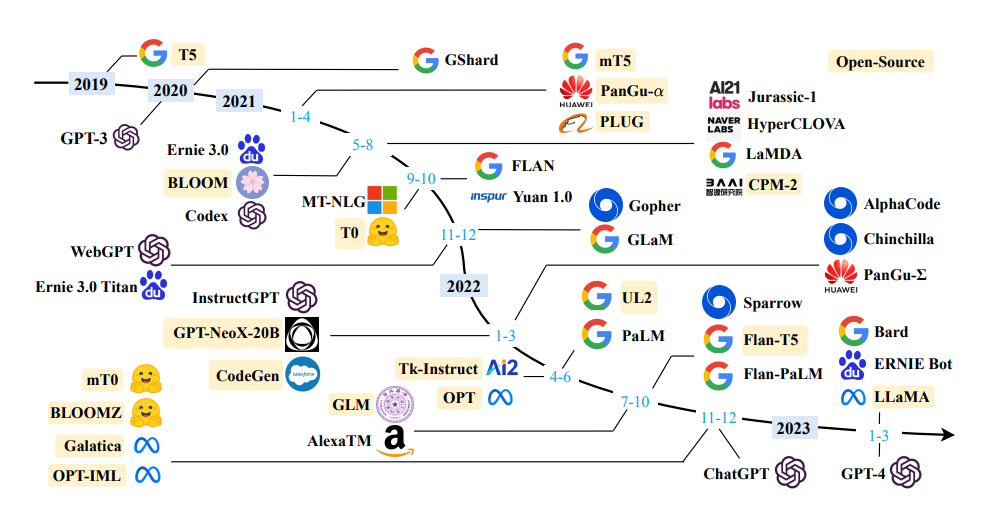
\includegraphics[width=\textwidth]{../img/neoantigen/llms}
	\end{figure}		
\end{frame}
%-------------------------------------------------------
%-------------------------------------------------------

%%%%%%%%%%%%%%%%%%%%%%%%%%%%%%%%%%%%%%%%%%%%%%%%%%%%%%%%%%%%%%%%%%%%%%%%%%%%%%%%%%%%%%%%%%%%%%%%%%%%%%%%%%%%%%%%
%%%%%%%%%%%%%%%%%%%%%%%%%%%%%%%%%%%%%%%%%%%%%%%%%%%%%%%%%%%%%%%%%%%%%%%%%%%%%%%%%%%%%%
\section{Review}
%%%%%%%%%%%%%%%%%%%%%%%%%%%%%%%%%%%%%%%%%%%%%%%%%%%%%%%%%%%%%%%%%%%%%%%%%%%%%%%%%%%%%%%%%%%%%%%%%%%%%%%%%%%%%%%%
%%%%%%%%%%%%%%%%%%%%%%%%%%%%%%%%%%%%%%%%%%%%%%%%%%%%%%%%%%%%%%%%%%%%%%%%%%%%%%%%%%%%%%


%-------------------------------------------------------
%-------------------------------------------------------
\begin{frame}{Inmunoterapia del Cáncer}{Pipeline}	
	\begin{figure}
		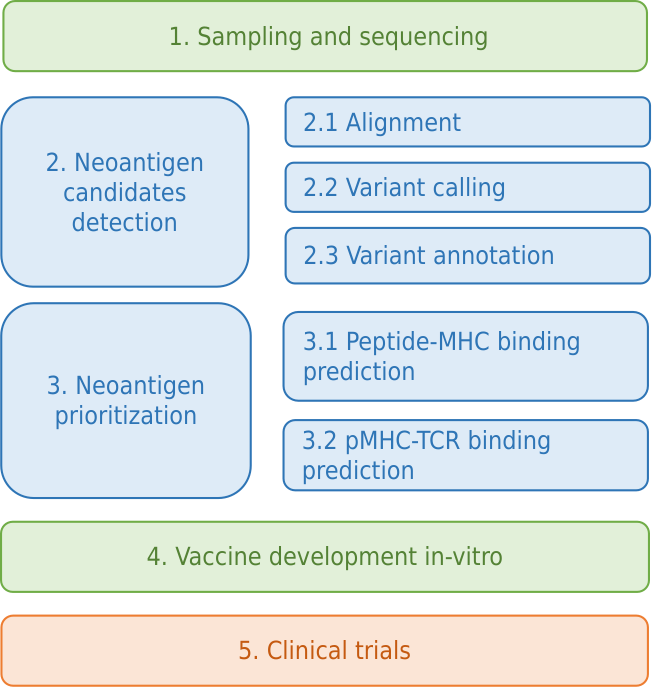
\includegraphics[width=0.6\textwidth]{../img/neoantigen/pipeline_ingles}
	\end{figure}		
\end{frame}
%-------------------------------------------------------
%-------------------------------------------------------

%-------------------------------------------------------
%-------------------------------------------------------
\begin{frame}{Inmunoterapia del Cáncer}{Pipeline}	
	\begin{figure}
		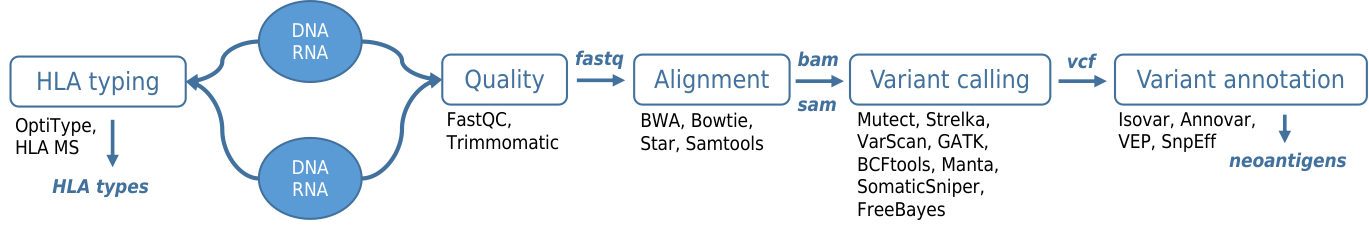
\includegraphics[width=\textwidth]{../img/neoantigen/neo_detection}
	\end{figure}		
\end{frame}
%-------------------------------------------------------
%-------------------------------------------------------

%-------------------------------------------------------
%-------------------------------------------------------
\begin{frame}{Inmunoterapia del Cáncer}{pMHC}	
	\begin{figure}
		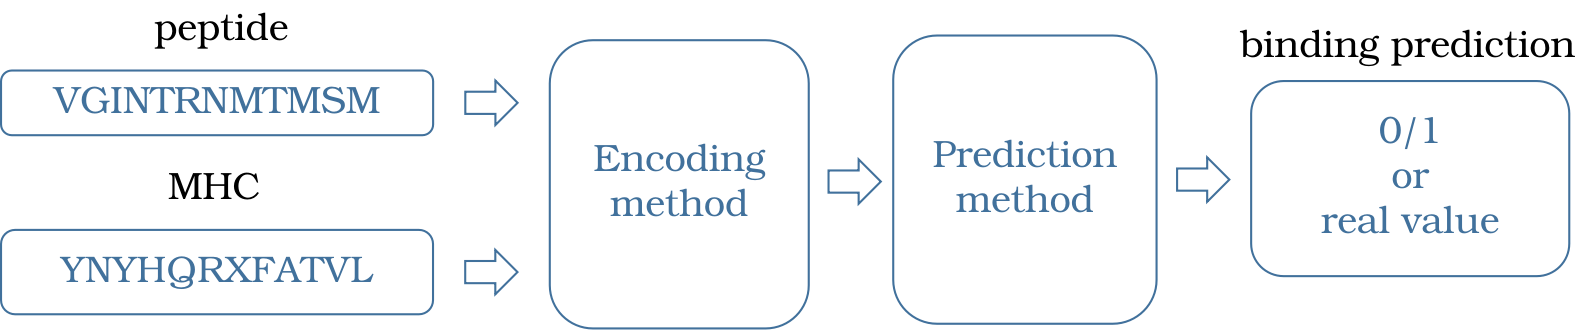
\includegraphics[width=\textwidth]{../img/neoantigen/pMHC}
	\end{figure}		
\end{frame}
%-------------------------------------------------------
%-------------------------------------------------------

%-------------------------------------------------------
%-------------------------------------------------------
\begin{frame}{Protein Language Models}{}	
	\begin{table}[h]%
		\centering
		\scriptsize
		\caption{Pre-trainned BERT models for several protein tasks: TAPE, ProtBert, ESM1, and ESM-2.}%
		
		\label{tab:pretrained}
		
		\setlength{\tabcolsep}{0.5em} % for the horizontal padding
		{\renewcommand{\arraystretch}{1.1}% for the vertical padding
			\scriptsize
			\begin{tabular}{lllllll}
				
				\textbf{Model}   & \textbf{Dataset} & \textbf{Samples} & \textbf{Layers} & \textbf{Hidden size} & \textbf{Att. heads} & \textbf{Params.} \\ \hline
				
				TAPE             & Pfam             & 30M                   & 12              & 768                  & 12                       & 92M                 \\
				ProtBert-BFD     & BFD              & 2122M                 & 30              & 1024                 & 16                       & 420M                \\
				
				ProtT5-XL     & Uniref50, BFD              & 2122M                 & 24              & 1024                 & 32                       & 3B                \\
				
				ProtT5-XXL     & Uniref50, BFD              & 2122M                 & 24              & 1024                 & 128                       & 11B                \\
				
				
				
				ESM-1 (6 layers)  & Uniref50         & 60M                   & 6               & 768                  & 12                       & 43M                  \\
				ESM-1 (12 layers)  & Uniref50         & 60M                   & 12               & 768                  & 12                       & 85M                  \\
				ESM-1 (34 layers)  & Uniref50         & 60M                   & 34               & 1280                  & 20                       & 670M                  \\
				ESM-1b  & Uniref50         & 60M                   & 34               & 1280                  & 20                       & 650M                  \\
				
				ESM-2 (6 layers)  & Uniref50         & 60M                   & 6               & 320                  & 20                       & 8M                  \\
				ESM-2 (12 layers)  & Uniref50         & 60M                   & 12              & 480                  & 20                       & 35M                 \\
				ESM-2 (30 layers) & Uniref50         & 60M                   & 30              & 640                  & 20                       & 150M                \\
				ESM-2 (33 layers)  & Uniref50         & 60M                   & 33              & 1280                 & 20                       & 650M               \\
				
				ESM-2 (36 layers)  & Uniref50         & 60M                   & 36              & 2560                 & 20                       & 3B               \\
				
				ESM-2 (48 layers)  & Uniref50         & 60M                   & 48              & 5120                 & 20                       & 15B               \\
				
		\end{tabular}}
		
	\end{table}
			
\end{frame}
%-------------------------------------------------------
%-------------------------------------------------------

%-------------------------------------------------------
%-------------------------------------------------------
\begin{frame}{Fin-tuning}{pMHC}	
	\begin{figure}
		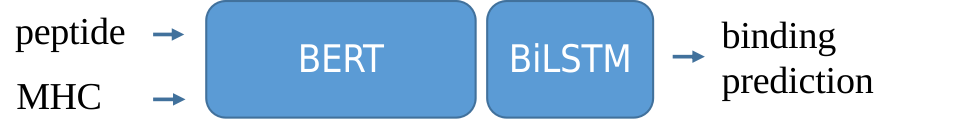
\includegraphics[width=\textwidth]{../img/proposal/pMHC}
	\end{figure}		
\end{frame}
%-------------------------------------------------------
%-------------------------------------------------------

%-------------------------------------------------------
%-------------------------------------------------------
\begin{frame}{Transformer models used in pMHC}{}	
%\begin{comment}
\begin{table}[h]
	
	\caption{Transformers and deep learning methods with attention mechanism used for pMHC binding prediction.}
	\label{tab:transformes}
	\setlength{\tabcolsep}{0.5em} % for the horizontal padding
	{\renewcommand{\arraystretch}{1.1}% for the vertical padding
		\tiny
		%\begin{scriptsize}
		\begin{tabular}{p{1cm}p{1cm}p{1cm}p{6cm}}
			\multicolumn{1}{l}{\textbf{Year}}                                   & \textbf{Name}             & \textbf{Input}            & \textbf{Model}     \\  \hline
			
			2023\cite{hashemi2023improved}&	ESM-GAT  &	One-hot & BERT with transfer learning from ESM1b and ESM2 fine-tuned with a Graph Attention Network (GAT) at the end. It outperformed NetMHCpan4.1.	\\
			
			
			2023\cite{kalemati2023capsnet}&	CapsNet-MHC&	BLOSUM62 & Capsule Neural Network, it outperformed state-of-art tools for small peptides of 8 to 11-mer.	\\
			
			2023\cite{ye2023stmhcpan}&	STMHCpan  &	One-hot & A Star-Transformer model, it use usefull for anylenght peptides and could extended for predicting T-cell responses.	\\
			
			2023\cite{jing2023dapnet}&	DapNet-HLA&	Fused word embedding & Combined the advantages of CNN, SENet (for pooling), and LSTM with attention.	\\
			
			2022\cite{zhang2022hlab}&	HLAB&	One-hot & BERT from ProtBert pre-trained model followed by a BiLSTM with attention mechanism.	\\
			
			2022\cite{wang2022mhcroberta}          & MHC RoBERTa            & One-hot &  RoBERTa  pre-trained and followed by 12 multi-head SA and a FC layers, it outperformed NetMHCPan 3.0.                                                                                          \\
			2022\cite{chu2022transformer}          & TransPHLA             & One-hot         & It used SA mechanism based on four blocks, it slightly outperformed NetMHCpan4.1 and is faster making predictions.\\
			
			2021\cite{chen2021jointly}  & CapTransformer            & One-hot   &  Transformer with cross attention pooling to capture local and global information.  \\
			
			2021\cite{gasser2021interpreting}  & ImmunoBERT            & One-hot                     & BERT from TAPE pre-trained followed by a linear layer. Authors claimed that N-terminal and C-terminals are highly relevant after analysis with SHAP and LIME.   \\
			
			                   
		\end{tabular}
		%	\end{scriptsize}
}
\end{table}
	
\end{frame}
%-------------------------------------------------------
%-------------------------------------------------------

%%%%%%%%%%%%%%%%%%%%%%%%%%%%%%%%%%%%%%%%%%%%%%%%%%%%%%%%%%%%%%%%%%%%%%%%%%%%%%%%%%%%%%%%%%%%%%%%%%%%%%%%%%%%%%%%
%%%%%%%%%%%%%%%%%%%%%%%%%%%%%%%%%%%%%%%%%%%%%%%%%%%%%%%%%%%%%%%%%%%%%%%%%%%%%%%%%%%%%%
\section{Conclusiones}
%%%%%%%%%%%%%%%%%%%%%%%%%%%%%%%%%%%%%%%%%%%%%%%%%%%%%%%%%%%%%%%%%%%%%%%%%%%%%%%%%%%%%%%%%%%%%%%%%%%%%%%%%%%%%%%%
%%%%%%%%%%%%%%%%%%%%%%%%%%%%%%%%%%%%%%%%%%%%%%%%%%%%%%%%%%%%%%%%%%%%%%%%%%%%%%%%%%%%%%


%-------------------------------------------------------
%-------------------------------------------------------
\begin{frame}{Conclusiones}{}
	\begin{block}{}
		Con el auge de los Transformers, cada vez se desarrollan mas propuestas de fine-tuning para diversas areas en Proteómica.
	\end{block}


	\begin{block}{}
		Se ha mejorado mucho el acierto para la detección de neo antígenos; sin embargo la gran variedad de tipos de Cancer aún es una tarea muy compleja.
	\end{block}

	\begin{block}{}
		Entrenar estos modelos implica un alto costo computacional lo cual dificulta la investigación de laboratorios perqueños.
	\end{block}
\end{frame}
%-------------------------------------------------------
%-------------------------------------------------------

%-------------------------------------------------------
%-------------------------------------------------------
\begin{frame}[allowframebreaks]
	\frametitle{References}
	%\bibliographystyle{amsalpha}
	\bibliographystyle{IEEEtran}
	\bibliography{../bibliography_thesis.bib}
\end{frame}
%-------------------------------------------------------
%-------------------------------------------------------

%-------------------------------------------------------
%-------------------------------------------------------
\if\mycmd1 % MY THEME
\1{
	{\1
		\begin{frame}[plain,noframenumbering]
			%\finalpage{Thank you}
			\begin{figure}[]
				\centering
				
\includegraphics[width=\textwidth,height=0.7\textheight,keepaspectratio]{img/question.png}
				%\label{img:mot2}
				%\caption{Image example in 2 gray levels.}
			\end{figure}
	\end{frame}}
	\else % CS THEME
	\begin{frame}{Questions?}
		\begin{figure}[]
			\centering
			
\includegraphics[width=\textwidth,height=0.7\textheight,keepaspectratio]{img/question.png}
			%\label{img:mot2}
			%\caption{Image example in 2 gray levels.}
		\end{figure}
		
	\end{frame}
	\fi
	%-------------------------------------------------------
	%-------------------------------------------------------
	

\end{document}